% generated by research/frisos-sturm/figura_hl.py (Curiosity); do not edit by hand
\begin{figure}[H]
\centering
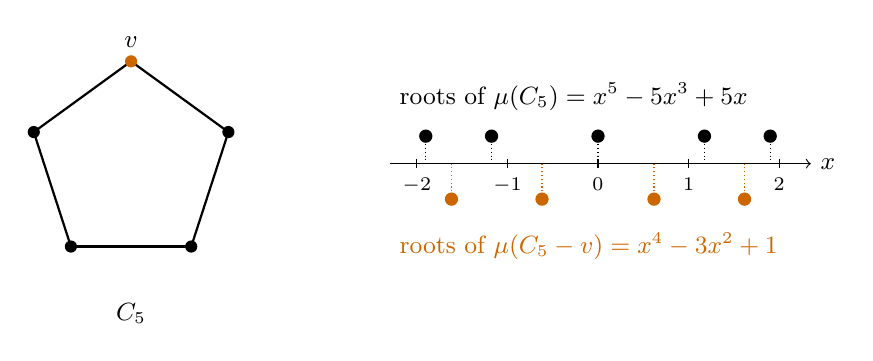
\begin{tikzpicture}[every node/.style={font=\small}]
  \draw[thick] (0.000,1.300) -- (-1.236,0.402);
  \draw[thick] (-1.236,0.402) -- (-0.764,-1.052);
  \draw[thick] (-0.764,-1.052) -- (0.764,-1.052);
  \draw[thick] (0.764,-1.052) -- (1.236,0.402);
  \draw[thick] (1.236,0.402) -- (0.000,1.300);
  \fill[fill=orange!80!black] (0.000,1.300) circle (2.2pt);
  \fill[fill=black] (-1.236,0.402) circle (2.2pt);
  \fill[fill=black] (-0.764,-1.052) circle (2.2pt);
  \fill[fill=black] (0.764,-1.052) circle (2.2pt);
  \fill[fill=black] (1.236,0.402) circle (2.2pt);
  \node[above] at (0.000,1.350) {$v$};
  \node at (0,-1.9) {$C_5$};
  \draw[->] (3.285,0) -- (8.633,0) node[right] {$x$};
  \draw (3.630,0.06) -- (3.630,-0.06) node[below] {\scriptsize $-2$};
  \draw (4.780,0.06) -- (4.780,-0.06) node[below] {\scriptsize $-1$};
  \draw (5.930,0.06) -- (5.930,-0.06) node[below] {\scriptsize $0$};
  \draw (7.080,0.06) -- (7.080,-0.06) node[below] {\scriptsize $1$};
  \draw (8.230,0.06) -- (8.230,-0.06) node[below] {\scriptsize $2$};
  \fill (3.743,0.35) circle (2.4pt);
  \draw[densely dotted] (3.743,0.35) -- (3.743,0);
  \fill (4.578,0.35) circle (2.4pt);
  \draw[densely dotted] (4.578,0.35) -- (4.578,0);
  \fill (5.930,0.35) circle (2.4pt);
  \draw[densely dotted] (5.930,0.35) -- (5.930,0);
  \fill (7.282,0.35) circle (2.4pt);
  \draw[densely dotted] (7.282,0.35) -- (7.282,0);
  \fill (8.117,0.35) circle (2.4pt);
  \draw[densely dotted] (8.117,0.35) -- (8.117,0);
  \fill[orange!80!black] (4.069,-0.45) circle (2.4pt);
  \draw[densely dotted, orange!80!black] (4.069,-0.45) -- (4.069,0);
  \fill[orange!80!black] (5.219,-0.45) circle (2.4pt);
  \draw[densely dotted, orange!80!black] (5.219,-0.45) -- (5.219,0);
  \fill[orange!80!black] (6.641,-0.45) circle (2.4pt);
  \draw[densely dotted, orange!80!black] (6.641,-0.45) -- (6.641,0);
  \fill[orange!80!black] (7.791,-0.45) circle (2.4pt);
  \draw[densely dotted, orange!80!black] (7.791,-0.45) -- (7.791,0);
  \node[anchor=west] at (3.285,0.85) {roots of $\mu(C_5) = x^5 - 5x^3 + 5x$};
  \node[anchor=west, orange!80!black] at (3.285,-1.05) {roots of $\mu(C_5 - v) = x^4 - 3x^2 + 1$};
\end{tikzpicture}
\caption{The matching polynomial of the 5-cycle and of the path obtained by deleting the vertex $v$: all roots are real (Theorem \texttt{heilmann\_lieb}) and they interlace, which is the cone property used in the induction. The roots are $0, \pm\sqrt{(5\pm\sqrt5)/2}$ and $\pm(\sqrt5\pm1)/2$.}
\label{fig:example}
\end{figure}
